\documentclass[10pt,a4paper]{article}
\usepackage[margin=16mm,top=17mm,bottom=18mm,headheight=14pt,footskip=9mm]{geometry}
\usepackage{fontspec,xeCJK}
\defaultfontfeatures{}
\setmainfont[Path=C:/Windows/Fonts/,BoldFont=timesbd.ttf,ItalicFont=timesi.ttf,BoldItalicFont=timesbi.ttf]{times.ttf}
\setsansfont[Path=C:/Windows/Fonts/,BoldFont=arialbd.ttf]{arial.ttf}
\setmonofont[Path=C:/Windows/Fonts/]{consola.ttf}
\setCJKmainfont[Path=C:/Windows/Fonts/,FontIndex=0,BoldFont=msjhbd.ttc]{msjh.ttc}
\setCJKsansfont[Path=C:/Windows/Fonts/,FontIndex=0,BoldFont=msjhbd.ttc]{msjh.ttc}
\setCJKmonofont[Path=C:/Windows/Fonts/,FontIndex=0]{msjh.ttc}
\usepackage{amsmath,amssymb}
\usepackage{graphicx,xcolor,tabularx,array}
\usepackage{tikz}
\usetikzlibrary{arrows.meta}
\usepackage{fancyhdr}
\usepackage[unicode,colorlinks=true,urlcolor=blue]{hyperref}
\hypersetup{pdftitle={Lab 1: Temporal Difference Learning for 2048},pdfauthor={唐予安 315551017}}
\definecolor{ink}{HTML}{172B40}
\definecolor{blue}{HTML}{246B9C}
\definecolor{orange}{HTML}{CC6A20}
\definecolor{light}{HTML}{EDF3F7}
\color{ink}
\pagestyle{fancy}\fancyhf{}
\fancyhead[L]{\sffamily\scriptsize NYCU / REINFORCEMENT LEARNING / FALL 2026}
\fancyfoot[L]{\scriptsize Lab 1 | Temporal Difference Learning for 2048}
\fancyfoot[R]{\thepage}
\renewcommand{\headrulewidth}{0pt}
\renewcommand{\footrulewidth}{0.3pt}
\setlength{\parindent}{0pt}\setlength{\parskip}{5pt}
\renewcommand{\baselinestretch}{1.12}
\setlength{\abovedisplayskip}{7pt}\setlength{\belowdisplayskip}{7pt}
\setlength{\emergencystretch}{2em}
\newcommand{\reporttitle}[2]{\vspace*{2mm}{\sffamily\bfseries\LARGE #1}\par\vspace{3pt}{\small #2}\par\vspace{6pt}}
\newcommand{\topic}[1]{\par\vspace{5pt}{\sffamily\bfseries\large\color{blue}#1}\par\vspace{2pt}}
\newcommand{\toprule}{\hline}\newcommand{\midrule}{\hline}\newcommand{\bottomrule}{\hline}
\newcolumntype{Y}{>{\raggedright\arraybackslash}X}
\begin{document}


\reporttitle{Lab 1：2048 的時序差分學習}{TD-state 與 TD-after-state 的實作及實驗比較}

姓名：唐予安　　學號：315551017　　實驗日期：2026/09/24\par

\topic{摘要}

本實驗以課程提供的 2048\_sample.cpp 為基礎，使用四組 6-tuple network，分別學習移動前狀態價值 \(V_s(s)\) 與移動後狀態價值 \(V_a(s^{\prime})\)。兩版皆從零權重訓練 100,000 局，再凍結權重評估 1,000 局。TD-state 的 2048 達成率為 79.1\%，TD-after-state 為 76.7\%；後者的平均分數較高，且訓練時間較短。兩項效能指標呈現不同排序，顯示平均回報與達成特定方塊的機率並不等價。\par

\topic{1. 遊戲環境與狀態定義}

棋盤為 4 \(\times\) 4。動作為上、右、下、左；無法改變棋盤的動作不合法。相同數值方塊合併時，新方塊數值即為 reward，多次合併的 reward 相加。每次合法移動後，從空格均勻選一格，以 0.7 機率產生 2、0.3 機率產生 4。遊戲持續至無合法動作，並不在首次取得 2048 時結束。\par

\[s\xrightarrow{a,\,r}s^{\prime}\xrightarrow{\text{隨機 popup}}s^{\prime\prime}.\]

s 為 before-state；\(s^{\prime}\) 為合併完成、尚未 popup 的 after-state；\(s^{\prime\prime}\) 為下一個 before-state。本文的 \(V_s\) 與 \(V_a\) 分別指兩個版本各自訓練的 n-tuple 價值函數。\par

\topic{2. 實驗設定}

{\small\renewcommand{\arraystretch}{1.35}\begin{tabularx}{\linewidth}{@{}YY@{}}\toprule

項目 & 共同設定 \\\midrule

訓練 / 評估 & 每版 100,000 / 1,000 局；評估時不更新權重 \\

學習設定 & TD(0)，\(\alpha=0.1\)；無額外折扣（\(\gamma=1\)） \\

網路與初始值 & 4 \(\times\) 6-tuples，每組 8 種對稱；所有權重初始為 0 \\

隨機種子 & 訓練 42；評估 2026 \\

動作與更新 & greedy 選擇；每局結束後由後向前更新 \\

執行環境 & Windows，MSYS2 g++ 15.2.0，C++11，-O3 \\

\bottomrule\end{tabularx}\par}

{\small 兩版各使用單執行緒 CPU，同時啟動；未使用 GPU 或 -march=native。計時包含局內模擬、更新及中途 checkpoint，不含最終權重寫檔；不是專用機器上的隔離效能基準。\par}

\clearpage

\reporttitle{價值函數：n-tuple network}{表示方式、對稱共享與權重更新}

\topic{3. 棋盤編碼與特徵設計}

沿用 sample 的 64-bit bitboard：每格以 4 bits 記錄指數，0 表示空格，1 表示 2，2 表示 4。格子以 row-major 編為 0 至 15。直接建立完整棋盤價值表過大，因此用數個局部 pattern 的查表結果相加，近似整體棋盤價值。\par

{\small\renewcommand{\arraystretch}{1.35}\begin{tabularx}{\linewidth}{@{}YYY@{}}\toprule

Pattern & 格子索引（十進位） & 權重表 \\\midrule

P1 & 0, 1, 2, 3, 4, 5 & \(16^6\) 個 float \\

P2 & 4, 5, 6, 7, 8, 9 & \(16^6\) 個 float \\

P3 & 0, 1, 2, 4, 5, 6 & \(16^6\) 個 float \\

P4 & 4, 5, 6, 8, 9, 10 & \(16^6\) 個 float \\

\bottomrule\end{tabularx}\par}

每組 pattern 對四個旋轉方向與鏡射共取 8 種對稱，這 8 種對稱共用同一組 LUT。四組 pattern 各自擁有權重表，不互相共享。每組 \(16^6\) \(\times\) 4 bytes = 64 MiB，四組合計 256 MiB。\par

\topic{4. 索引與估值}

\begin{align*}
I_p(b)&=\sum_{j=0}^{5}b[p_j]\,16^j,\\
V(b)&=\sum_{p=1}^{4}\sum_{g=1}^{8}w_p\!\left[I_{p,g}(b)\right].
\end{align*}

其中 b[i] 是格子 i 的指數；g 是一種旋轉或鏡射。索引實作使用位元位移與 OR，例如三格指數依序為 1、2、3，索引為十六進位 0x321。estimate() 將 32 個 active feature 的值相加。\par

\topic{5. TD-error 如何更新權重}

\begin{align*}
\delta&=y-V(b),\\
w_p\!\left[I_{p,g}(b)\right]&\leftarrow w_p\!\left[I_{p,g}(b)\right]+\frac{0.1}{32}\,\delta.
\end{align*}

其中 \(y\) 表示 TD-target。learning::update() 先把 \(\alpha\delta\) 分給四個 pattern；pattern::update() 再除以 8，更新對應 LUT。對稱特徵若指向同一 LUT 索引，該權重會收到多次梯度貢獻，因為估值總和中也多次使用它；不能直接把重複索引去除。回傳新估值時，在所有權重完成更新後重新計算。\par

{\small 共享局部特徵讓不同棋盤可共用已學到的資訊，但也會造成泛化干擾。對稱共享避免為等價旋轉另建模型，節省參數；本實驗沒有使用 CNN，也沒有額外 heuristic 或多步搜尋。\par}

\clearpage

\reporttitle{TD-state：學習 \(V_s(s)\)}{動作選擇使用期望值；學習使用實際轉移樣本}

\topic{6. 動作選擇}

對每個合法動作先得到 reward r 與 after-state \(s^{\prime}\)。若 \(s^{\prime}\) 有 k 個空格，逐一枚舉每個位置生成 2 或 4 的共 2k 種 next states。位置與數值的聯合機率分別為 0.7/k、0.3/k。\par

\begin{align*}
Q_s(s,a)&=r+\sum_{i\in\operatorname{empty}(s^{\prime})}
\left[\frac{0.7}{k}V_s(s^{\prime\prime}_{i,2})+\frac{0.3}{k}V_s(s^{\prime\prime}_{i,4})\right],\\
a^*&=\operatorname*{arg\,max}_{a\in A(s)} Q_s(s,a).
\end{align*}

終局候選的 \(V_s\) 明確視為 0。程式以 expected\_next\_value() 計算期望值，再由 \texttt{select\_\allowbreak best\_\allowbreak move()} 選出最大分數；相同分數時保留先遇到的動作，順序為上、右、下、左。\par

\topic{7. TD-target、TD-error 與 backup diagram}

\begin{center}\begin{tikzpicture}[>=Stealth,box/.style={draw=blue,fill=light,rounded corners,minimum width=29mm,minimum height=12mm,align=center,font=\small}]
\node[box] (a) at (0,0) {$s$\\待更新 $V_s$};
\node[box] (b) at (5.5,0) {$s^{\prime}$\\移動後棋盤};
\node[box] (c) at (11,0) {$s^{\prime\prime}$\\實際下一狀態};
\draw[->,blue] (a)--node[above,font=\small]{$a,r$}(b);
\draw[->,blue] (b)--node[above,font=\small]{popup}(c);
\draw[->,orange,thick] (c.south)--++(0,-.65)-|node[pos=.25,below,font=\small]{$y_s=r+V_s(s^{\prime\prime})$} (a.south);
\end{tikzpicture}\end{center}

{\small 圖 1．實線表示遊戲實際走過的單步轉移；橘色回傳箭頭表示更新 \(V_s(s)\) 的 TD backup。選動作時枚舉所有 popup，但這個 backup 只用該局實際抽到的 \(s^{\prime\prime}\)。\par}

\begin{align*}
y_s&=\begin{cases}r,&s^{\prime\prime}\text{ 為終局},\\r+V_s(s^{\prime\prime}),&\text{其他情況},\end{cases}\\
\delta_s&=y_s-V_s(s).
\end{align*}

TD(0) 使用一步 reward 加上下一狀態的估值作為 target，稱為 bootstrapping；不必等待完整 Monte Carlo return。正 TD-error 提升本次狀態相關權重，負 TD-error 則降低權重。\par

\topic{8. 程式實作與終局處理}

每局記錄 before-state、after-state、動作與 reward，最後附上無合法動作的 terminal sentinel。update\_episode() 由最後一個有效動作往前更新。current.before\_state() 是待訓練棋盤，next.before\_state() 是實際下一狀態；若 next 無效，後續價值設為 0，不把 sentinel 的 reward = -1 當成遊戲獎勵。\par

{\small 反向掃描時使用更新當下的估值，較後面的轉移可能已更新共享權重。因此這是講義指定的 modified backward training，而不是凍結一整局 target 後再一次更新。\par}

\clearpage

\reporttitle{TD-after-state：學習 \(V_a(s^{\prime})\)}{移動後估值與反向更新時的 greedy 重新選擇}

\topic{9. 動作選擇}

\begin{align*}
Q_a(s,a)&=r+V_a(s^{\prime}),\\
a^*&=\operatorname*{arg\,max}_{a\in A(s)}Q_a(s,a).
\end{align*}

\(V_a(s^{\prime})\) 學習移動完成後的預期後續回報，因此當前動作的 reward r 不包含在 \(V_a(s^{\prime})\) 中。選動作時，每個合法動作只需對其 after-state 估值，不必展開所有 popup 分支。\par

\topic{10. TD-target、TD-error 與 backup diagram}

\begin{center}\begin{tikzpicture}[>=Stealth,box/.style={draw=blue,fill=light,rounded corners,minimum width=29mm,minimum height=12mm,align=center,font=\small}]
\node[box] (a) at (0,0) {$s^{\prime}$\\待更新 $V_a$};
\node[box] (b) at (5.5,0) {$s^{\prime\prime}$\\實際 popup};
\node[box] (c) at (11,0) {$s^{\prime}_{\mathrm{next}}$\\greedy 下一步};
\draw[->,blue] (a)--node[above,font=\small]{popup}(b);
\draw[->,blue] (b)--node[above,font=\small]{$a_{\mathrm{next}},r_{\mathrm{next}}$}(c);
\draw[->,orange,thick] (c.south)--++(0,-.65)-|node[pos=.25,below,font=\small]{$y_a=r_{\mathrm{next}}+V_a(s^{\prime}_{\mathrm{next}})$} (a.south);
\end{tikzpicture}\end{center}

{\small 圖 2．先從 \(s^{\prime}\) 經由實際 popup 得到 \(s^{\prime\prime}\)，再用目前權重重新選擇下一個 greedy action。橘色箭頭將下一個動作 reward 與其 after-state 估值回傳至 \(V_a(s^{\prime})\)。\par}

\begin{align*}
a_{\mathrm{next}}&=\operatorname*{arg\,max}_{a\in A(s^{\prime\prime})}
\bigl[r_{\mathrm{next}}+V_a(s^{\prime}_{\mathrm{next}})\bigr],\\
y_a&=r_{\mathrm{next}}+V_a(s^{\prime}_{\mathrm{next}}),\\
\delta_a&=y_a-V_a(s^{\prime}).
\end{align*}

如果 \(s^{\prime\prime}\) 沒有合法動作，\(y_a=0\)。注意 target 中使用的是下一步 reward \(r_{\mathrm{next}}\)，不是形成目前 \(s^{\prime}\) 的 reward r；後者已經在上一個動作的評分中計入。\par

\topic{11. 更新流程與兩版差異}

update\_episode() 同樣由後往前處理；以 current.after\_state() 為待訓練棋盤，對 next.before\_state() 呼叫 \texttt{select\_\allowbreak best\_\allowbreak move()}，使用目前權重算出的 greedy.value() 作為 target。既不沿用 path 內過時的 value，也不強制沿用當時實際選過的下一步動作。\par

{\small TD-after-state 把隨機 popup 的影響吸收到學得的價值函數，降低選動作的估值次數。這並不保證每項遊戲指標都較高，最終仍須以相同訓練量和獨立評估比較。\par}

\clearpage

\reporttitle{實驗結果}{每版 100,000 局訓練；凍結權重後各評估 1,000 局}

\topic{12. 平均分數訓練曲線}

\begin{center}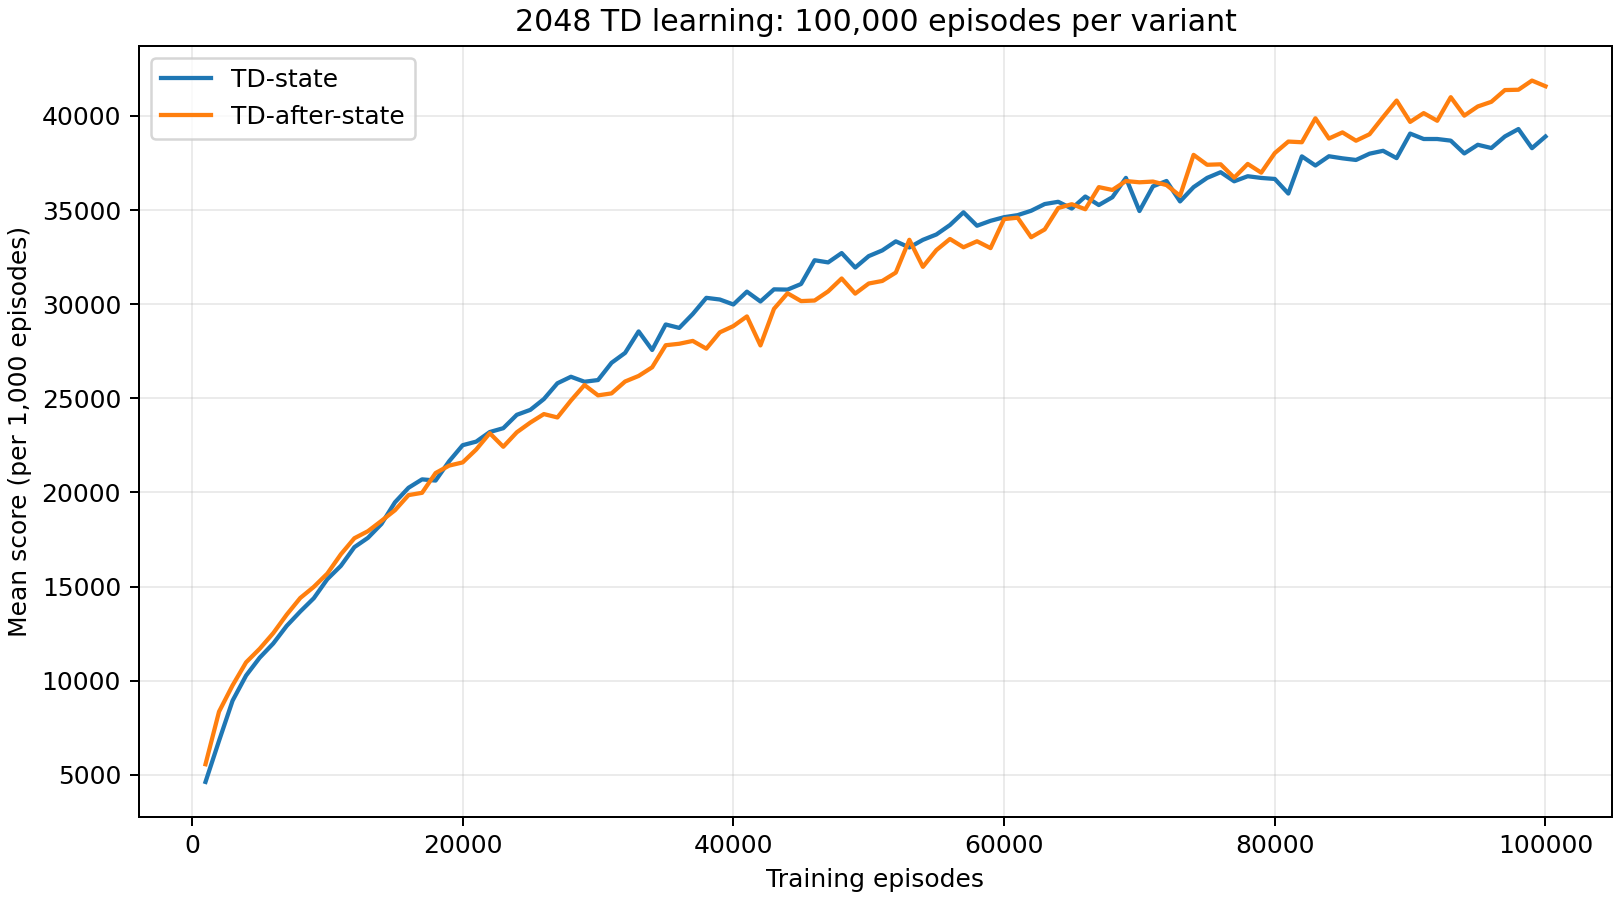
\includegraphics[width=\linewidth]{../../logs/training_curve_20260924_202933.png}\end{center}

{\small 圖 3．每個點為連續 1,000 局的平均分數，兩條曲線各包含 100 點。資料來自逐局訓練 CSV；未進行跨點平滑。此圖呈現訓練中的表現，不是凍結權重的測試曲線。\par}

\topic{13. 最終固定權重評估}

{\small\renewcommand{\arraystretch}{1.35}\begin{tabularx}{\linewidth}{@{}YYY@{}}\toprule

指標 & TD-state & TD-after-state \\\midrule

平均分數 & 39,824.82 & 41,554.47 \\

最高分數 & 138,256 & 130,600 \\

2048 達成局數 / 比例 & 791 / 1,000；79.1\% & 767 / 1,000；76.7\% \\

4096 達成率 & 27.3\% & 38.8\% \\

8192 達成率 & 1.0\% & 0.9\% \\

訓練時間（秒） & 1,160.38 & 413.85 \\

評估時間（秒） & 13.42 & 2.83 \\

\bottomrule\end{tabularx}\par}

{\small 達成率定義：終局最大方塊至少為指定數值的局數 / 全部評估局數。相同 seed 2026 用於兩版評估，但兩版策略會產生不同長度與棋盤的軌跡，不代表逐局環境完全配對。評估期間不更新權重，也沒有重新挑選測試種子。\par}

\clearpage

\reporttitle{分析、驗證與重現}{結果解讀、限制與提交內容}

\topic{14. 結果分析}

兩版曲線皆持續上升。TD-state 在中段的平均分數略高，約七萬局後 TD-after-state 逐漸領先；不能僅由這次曲線推論演算法的一般優劣。最終 TD-after-state 平均分數高約 4.34\%，且 4096 達成率高 11.5 個百分點；TD-state 的 2048 達成率則高 2.4 個百分點。\par

這個差異符合兩種指標衡量不同目標：平均分數計入合併獎勵與達成 2048 後的持續表現，而 2048 達成率只計是否過門檻。依本次結果，Demo 優先選 TD-state；但僅使用一組訓練種子與一組評估種子，尚不足以證明 2.4 個百分點差距穩定存在。\par

本次 TD-after-state 訓練約快 2.80 倍，評估約快 4.75 倍。合理原因是它不需枚舉 popup 的 2k 種結果；但兩程序曾同時執行，且遊戲長度不同，因此這些是本次端到端實測值，不是純演算法複雜度或隔離硬體效能比。\par

\topic{15. 正確性驗證與限制}

tests/run\_tests.py 通過兩版測試：tuple 索引、對稱及重複索引梯度、popup 機率、終局價值、動作排序、反向 target、after-state 重新 greedy、權重存取、checkpoint、固定 seed 重現與錯誤參數拒絕。C++11 搭配 -Wall -Wextra -Wpedantic 編譯無警告。訓練後來源檔 SHA-256 與啟動時紀錄一致。\par

{\small 棋盤沿用 sample 的 4-bit 格子，上限為 32768；若候選移動生成 65536，程式會明確停止而非靜默溢位。本次最大方塊為 8192，未觸發此限制。後續可增加評估種子、延長訓練或比較 pattern，但本文不把尚未執行的實驗當成結果。\par}

\topic{16. 重現方式與實驗產物}

兩檔均可獨立編譯：g++ -std=c++11 -O3 td\_state.cpp -o td\_state（另一版替換檔名）。訓練參數為 --episodes 100000 --alpha 0.1 --seed 42；搭配 --save、--log 與 --checkpoint-every 10000。評估參數為 --eval --load MODEL --episodes 1000 --seed 2026。詳細命令見 README.md。\par

{\small 本次 run ID：20260924\_202933。逐局紀錄、曲線、摘要及來源檔雜湊保存在 logs/；兩版最終權重保存在 models/。報告與 td\_state.cpp、td\_afterstate.cpp 應一同繳交，模型權重另留供 Demo 載入，不放入繳交壓縮檔。\par}

\topic{參考資料}

{\small [1] NYCU CGI Lab, Lab1-TD (2026).pdf，頁 1-4：作業需求、網路設定、modified backward training 與評分規定。

[2] NYCU CGI Lab, Lab1-Guide (2026).pdf，頁 6-18：state / after-state、TD backup、n-tuple 對稱與範例程式說明。

[3] 課程提供的 2048\_sample.cpp：bitboard、pattern、state 與 learning 架構。

[4] 本次實驗的 train / eval CSV 與 results\_20260924\_202933.json：所有數值與圖 3 的直接資料來源。\par}

\end{document}